% !TEX program = xelatex
% =============================================================================
%  2026 江苏省大学生机器人大赛技术报告
%  编译：xelatex MaiTechReport.tex  （连续跑两遍，目录与页码才稳定）
% =============================================================================
\documentclass{MaiTechReport}

% 照片占位框：图片到位后把 \MaiPhotoPlaceholder 换成 \includegraphics
\newcommand{\MaiPhotoPlaceholder}[2]{%
  \fbox{\parbox[c][#1][c]{0.82\textwidth}{\centering\songti\zihao{5}#2}}%
}

\begin{document}

% ---------------------------------------------------------------------------
% 封面（队伍信息）
% ---------------------------------------------------------------------------
\MaiCover
  {403 无人车多车交互赛}
  {南京理工大学}
  {踢踏舞}
  {张冠良\quad 肖通\quad 张子傲}
  {樊卫华 fanweihua@njust.edu.cn}
  {2026.10.28}

% ---------------------------------------------------------------------------
% 技术报告使用授权说明
% 签名页扫描件放到 MaiFigs/Mai授权页扫描.pdf 后会自动整页替换
% ---------------------------------------------------------------------------
\MaiAuthorization

% ---------------------------------------------------------------------------
% 中文摘要
% ---------------------------------------------------------------------------
\MaiChineseAbstract
  {基于灰度视觉与多传感器融合的无人车多车交互系统设计与实现}
  {张冠良\quad 肖通\quad 张子傲\\
   （南京理工大学 自动化学院，江苏 南京 210094）}
  {本文面向 2026 江苏省大学生机器人大赛 403 无人车多车交互赛，设计并实现了一辆以 TC264D 双核微控制器为核心的自主无人车。系统以 120$\times$70 灰度摄像头为主要感知器件，完成赛道边界提取、双车道识别、锥形标检测与道路标线识别；以 DL1B 激光测距模块实现非接触式发车；以 WiFi SPI 模块建立 UDP 调试日志通道。控制层采用变增益位置式 PD 转向控制与增量式 PID 速度闭环。针对双车道虚线断口导致的赛道宽度跳变，提出宽度归一化与迟滞选道策略；针对反光、人行横道造成的边界污染，提出不可信帧保持策略；针对红色锥形标在灰度图中与车道线同为白色的特点，提出基于白段宽度的二维 blob 检测与锁存式绕行方法。实车调试表明，所提方法能够改善双车道循迹的稳定性，锥形标绕行已能基本完成；减速标线识别与人行横道停车逻辑已实现，仍需结合场地光照继续整定；同时实现了基于左右半车道白点占比的超车/会车状态机，默认关闭以便现场标定。}
  {无人车；灰度视觉；锥形标识别；PID 控制；多传感器融合}

% ---------------------------------------------------------------------------
% 英文摘要
% ---------------------------------------------------------------------------
\MaiEnglishAbstract
  {Design and Implementation of a Multi-Sensor Autonomous Vehicle for the 403 Multi-Vehicle Interaction Competition}
  {ZHANG Guanliang\quad XIAO Tong\quad ZHANG Zi'ao\\
   (School of Automation, Nanjing University of Science and Technology,\\
   Nanjing 210094, Jiangsu, China)}
  {This paper presents an autonomous vehicle for the 403 Multi-Vehicle Interaction Competition of the 2026 Jiangsu Provincial University Robot Competition. The system is built around a dual-core TC264D microcontroller, a 120$\times$70 grayscale camera, a DL1B time-of-flight sensor and a WiFi SPI module. A width-normalized lane policy with hysteresis, a ghost-frame holding strategy, a cone detection method based on white-run width and a marker state machine are proposed. The steering loop uses a variable-gain PD controller, while the speed loop uses an incremental PID controller. Experiments show that the proposed methods improve the stability of two-lane tracking and that cone bypass has been basically achieved; the deceleration-marking recognition and the five-second stop before the zebra crossing have been implemented and are still being tuned. A lane-half white-ratio based overtaking/oncoming state machine is also implemented and is disabled by default for field calibration.}
  {autonomous vehicle; grayscale vision; cone detection; PID control; sensor fusion}

% ---------------------------------------------------------------------------
% 目录
% ---------------------------------------------------------------------------
\MaiTableOfContents

% ===========================================================================
% 正文
% ===========================================================================
\setcounter{section}{-1}

\section{引言/综述}
\label{sec:intro}

\subsection{赛项背景与任务}
2026 江苏省大学生机器人大赛 403 无人车多车交互赛以 1:10 无人车为平台，考察车辆在结构化道路上的自主感知、决策与执行能力\upcite{rule2026}。本文的章节结构与排版按照大赛技术报告撰写规范执行\upcite{spec2023}。赛项分为上下半场：上半场为超车与会车，下半场为锥形标与道路标线识别，两项成绩共同决定总排名。

下半场比赛路段为 12 m 长、1.5 m 宽的双车道直道，单车道宽 45 cm，路面为黑色 PVC 塑胶地板，标线为白色胶带，线宽 2 cm，人行横道线宽 4 cm。路段上依次布置两组锥形标，每组 5$\sim$7 个，与道路中线约呈 30$^\circ$ 夹角；锥形标之后依次为两个菱形减速标线、停车线和人行横道线。参赛车辆需要在无人工干预的条件下沿锥形标围出的线路行驶，看到第一个菱形标线后逐渐减速，并在人行横道前的停车线处停车 5 s，再起步通过终点\upcite{rule2026}。

除赛道任务外，规则还对车辆提出若干硬性要求：车辆外形长、宽、高分别不超过 50 cm、30 cm、30 cm；前大灯、前后转向灯、后刹车灯位置合理且功能正常；开机后所有车灯常亮或闪烁不少于 3 s；发车必须采用挥手、遮挡等非接触方式，禁止遥控；比赛过程中不得触碰车辆。上述要求直接决定了本系统的传感器布置、车灯控制和发车逻辑。

\subsection{国内外发展现状}
智能车视觉循迹通常采用“灰度摄像头 + 二值化 + 边缘提取 + 中线拟合 + PID”的技术路线\upcite{zhuo2007}。该路线计算量小、实时性好，适合无 GPU 的嵌入式平台；缺点是对光照变化、地面反光和赛道断线敏感。为克服固定阈值的问题，Otsu 等学者提出了基于灰度直方图的自适应阈值方法\upcite{otsu1979}，其核心思想是最大化类间方差，使前景与背景尽可能分开。本文在 Otsu 思路上采用迭代直方图分割，并在阈值上叠加可在线整定的比例系数，以适应比赛现场的光照差异。

在锥形标等目标检测方面，基于卷积神经网络的 YOLO 系列方法具有较高的精度\upcite{redmon2016}，但其模型参数量和算力需求对 TC264 这类无神经网络加速器的微控制器并不友好。考虑到比赛用锥形标为红色、高 6$\sim$9 cm、表面贴有约 1 cm 宽的白色环带，本文利用其在灰度图中的亮度与宽度特征进行传统视觉检测，在不增加算力负担的前提下实现实时识别。

在车辆控制方面，位置式 PID 与增量式 PID 是智能车最常用的两类控制器\upcite{zhuo2007}。位置式 PID 直接输出控制量，适合转向舵机；增量式 PID 输出控制量增量，天然具有抗积分饱和能力，适合电机速度闭环。本文根据执行机构特点分别采用变增益位置式 PD 与增量式 PID，并在速度环中加入软起动，避免起步冲击。此外，模型预测控制等方法在无人驾驶车辆轨迹跟踪中也有广泛应用\upcite{gong2014}，但其在线优化计算量对本文的微控制器平台偏大，因此仍采用结构简单的 PID 方案。

\subsection{本文主要工作与创新点}
本文围绕 403 赛项的任务，完成以下工作：
\begin{enumerate}
  \item 设计以 TC264D 双核微控制器为核心、灰度摄像头与激光测距融合的硬件平台；
  \item 设计 CPU0 控制、CPU1 感知的双核任务划分与 5 ms/10 ms 中断调度；
  \item 提出双车道宽度归一化与迟滞选道策略，解决虚线断口导致的左右道穿梭；
  \item 提出不可信帧保持策略，抑制反光和人行横道造成的边界污染；
  \item 设计基于白段宽度的锥形标检测与锁存式绕行状态机；
  \item 设计道路标线识别与“减速—停车 5 s—再起步”状态机；
  \item 实现基于 ToF 新样本投票的非接触发车与 UDP 无线调试通道；
  \item 设计赛项一的车辆检测、超车/会车状态机与灯光联动。
\end{enumerate}

本文的主要创新点在于：用“宽度归一化 + 迟滞”而不是单一阈值解决双车道选道问题；用“沿用上一次可信目标点”而不是立即回中解决横道前的边界污染；用“白段宽度”而不是颜色解决红色锥形标在灰度图中的识别问题；用“锁存固定时长”而不是误差收敛解决锥形标绕行中的视觉反馈振荡问题。

\section{系统整体设计}
\label{sec:overall}

\subsection{总体架构}
系统按功能划分为感知层、决策层、执行层和调试层，整体架构如图~\ref{fig:arch} 所示。感知层由 MT9V034 灰度摄像头和 DL1B 激光测距模块组成，分别提供赛道图像和车头前方的距离信息。决策层为 Infineon TC264D 双核微控制器，负责图像处理、赛道识别、状态机决策和控制量计算。执行层包括转向舵机、左右直流电机、编码器和 8 路车灯。调试层由 IPS200 液晶屏、按键和 WiFi SPI 模块组成，用于现场显示、参数整定和日志回传。

\begin{figure}[htbp]
  \centering
  \begin{tikzpicture}[scale=0.92,transform shape,
    box/.style={draw,rounded corners,minimum width=2.7cm,minimum height=1.0cm,align=center,font=\zihao{5}},
    arr/.style={-{Latex[length=2mm]},thick}]
    \node[box] (cam)  at (0,2.6)  {MT9V034\\灰度摄像头};
    \node[box] (tof)  at (0,1.1)  {DL1B\\激光测距};
    \node[box,minimum width=3.4cm] (mcu) at (4.8,1.85) {TC264D 双核\\感知 / 决策};
    \node[box] (servo) at (9.6,3.2) {转向舵机};
    \node[box] (motor) at (9.6,1.85) {左右直流电机\\+ 编码器};
    \node[box] (light) at (9.6,0.5) {8 路车灯};
    \node[box] (wifi)  at (4.8,-0.3) {WiFi SPI\\调试 / 日志};
    \node[box] (ips)   at (4.8,-1.6) {IPS200 屏\\按键};
    \draw[arr] (cam) -- (mcu);
    \draw[arr] (tof) -- (mcu);
    \draw[arr] (mcu) -- (servo);
    \draw[arr] (mcu) -- (motor);
    \draw[arr] (mcu) -- (light);
    \draw[arr] (mcu) -- (wifi);
    \draw[arr] (mcu) -- (ips);
  \end{tikzpicture}
  \caption{系统整体架构}
  \label{fig:arch}
\end{figure}

\subsection{双核任务划分与实时调度}
TC264D 具有两个 TriCore 内核，本文按“时间关键任务放中断、计算密集任务放 CPU1”的原则划分任务。CPU0 负责 5 ms 控制中断、10 ms 灯光与发车判定、主循环中的按键扫描、屏幕刷新和 UDP 日志发送；CPU1 负责摄像头帧处理、ToF 采样和图像算法。两核通过全局变量和帧完成标志通信，CPU1 每处理完一帧将 \texttt{mt9v03x\_finish\_flag} 清零，CPU0 只在标志置位时读取最新结果，避免读写同一帧造成撕裂。

中断调度如表~\ref{tab:schedule} 所示。5 ms 中断承担转向舵机输出和速度闭环，是控制系统的核心节拍；10 ms 中断承担车灯闪烁和 ToF 发车投票。转向与速度分开在不同中断中执行，避免一次中断内计算量过大导致抖动。

\begin{table}[htbp]
  \centering
  \caption{中断与任务调度}
  \label{tab:schedule}
  \begin{tabular}{lll}
    \toprule
    周期 & 任务 & 说明 \\
    \midrule
    5 ms & 速度闭环、电机输出 & 编码器采样、增量式 PID、PWM 输出 \\
    5 ms & 转向控制 & 目标点计算、变增益 PD、舵机 PWM \\
    10 ms & 车灯控制 & 转向灯闪烁、刹车灯、大灯 \\
    10 ms & ToF 发车判定 & 消费新样本、12 点滑动窗口投票 \\
    帧同步 & 图像处理 & 二值化、边界提取、锥桶与标线识别 \\
    主循环 & 屏幕、按键、日志 & 人机交互与无线调试 \\
    \bottomrule
  \end{tabular}
\end{table}

\subsection{比赛流程与状态机}
车辆上电后首先进入初始化阶段：完成时钟、舵机中位、电机、编码器、ToF、摄像头、按键、车灯和 WiFi 初始化。初始化期间 8 路车灯全部点亮，满足规则“开机后所有车灯亮起超过 3 s”的要求。随后车辆进入待发车状态，转向舵机保持中位，电机不输出。

发车采用两种模式：比赛模式 \texttt{START\_MODE=1} 下，ToF 连续检测到挥手动作后置位 \texttt{start\_trigger}；调试模式 \texttt{START\_MODE=2} 下，上电 20 s 后自动发车，便于无裁判环境下调试。发车后 \texttt{Stop\_1} 置 1，车辆进入循迹状态，依次执行：

\begin{enumerate}
  \item 双车道循迹：根据左右边界计算目标点，PD 控制舵机；
  \item 第一组锥形标：识别到锥桶后向空间较大的一侧变道，锁存 1 s；
  \item 第二组锥形标：锥桶离开视野 1 s 后解除锁存，按新的空间关系回线；
  \item 菱形减速：连续 8 帧确认后进入慢行状态，速度降为 50\%；
  \item 人行横道：连续 15 帧确认且近端行号超过 45 后停车 5 s；
  \item 停车结束后回到循迹状态，驶过终点。
\end{enumerate}

\subsection{两赛项共用平台与代码分支}
赛项一（超车与会车）与赛项二共用底盘、摄像头、执行机构和调试系统，差异主要在决策层：赛项一需要识别同向龟行车辆和对向车辆，判断可借道区间，控制转向灯与前大灯，并在超车后回到原车道；赛项二则需要识别锥形标和道路标线。本文的软件框架将“感知结果”和“行为决策”分离，图像处理和目标检测输出统一的结构体，行为层根据当前赛项选择状态机。

本轮提交两套独立工程：赛项二代码在 \texttt{bizhang\_1108}，重点实现双车道循迹、锥桶绕行与标线识别；赛项一代码在 \texttt{chaoche2024\_1109}，沿用同一套图像处理与边界提取思路，新增 \texttt{Car\_Scan()} 车辆检测和 \texttt{Overtake\_Control()} 超车/会车状态机。赛项一总开关 \texttt{OVERTAKE\_ENABLE} 默认 0，需现场标定车辆检测阈值后开启，详细实现见 4.12 节。

\subsection{主要创新点}
本文的创新点可概括为以下五点：
\begin{enumerate}
  \item \textbf{宽度归一化与迟滞选道}：把“检测到的宽度”分为单道与整条路两种模式，分别计算本道中心、左道中心和右道中心，并用 85/60 px 的迟滞门限避免模式抖动；
  \item \textbf{不可信帧保持}：当边界贴边、可信行不足或目标点越界时，沿用上一次可信目标点，连续 2 s 不可信才回中位；
  \item \textbf{锥形标锁存绕行}：用白段宽度而非颜色识别锥桶，用固定 1 s 锁存而非误差收敛完成一次变道，用“锥桶离开 1 s”判定一组结束；
  \item \textbf{非接触发车}：只消费 ToF 的新测量样本，过滤 8192 无效值，用“1 s 前方空旷布防 + 12 样本 8 命中”投票发车；
  \item \textbf{赛项一超车/会车状态机}：用左右半车道白点占比检测前车与对向车，按 IDLE $\to$ GO $\to$ BACK 固定时序完成借道、回线与灯光联动。
\end{enumerate}

\section{机械结构设计}
\label{sec:mech}

\subsection{底盘与总体布局}
车模采用逐飞科技 C 车模，前轮由 SU400 舵机通过拉杆转向，后轮由两个有刷直流电机驱动。整车实测外形尺寸为 29 cm$\times$18.5 cm$\times$25 cm（长$\times$宽$\times$高），满足规则“长不超过 50 cm、宽不超过 30 cm、高不超过 30 cm”的资格要求。车模原厂状态的竖直安装杆高约 35 cm，超出高度限制 5 cm；由于摄像头实际安装高度约 25 cm，本文将杆体上部截短，使整车高度降到约 25 cm，既保留了摄像头视野，又通过了资格评定。主控板、摄像头、ToF、WiFi 模块、IPS200 屏和电池沿车体纵向布置，电池靠近车体中部以降低重心，减少加减速时的俯仰。

\begin{figure}[htbp]
  \centering
  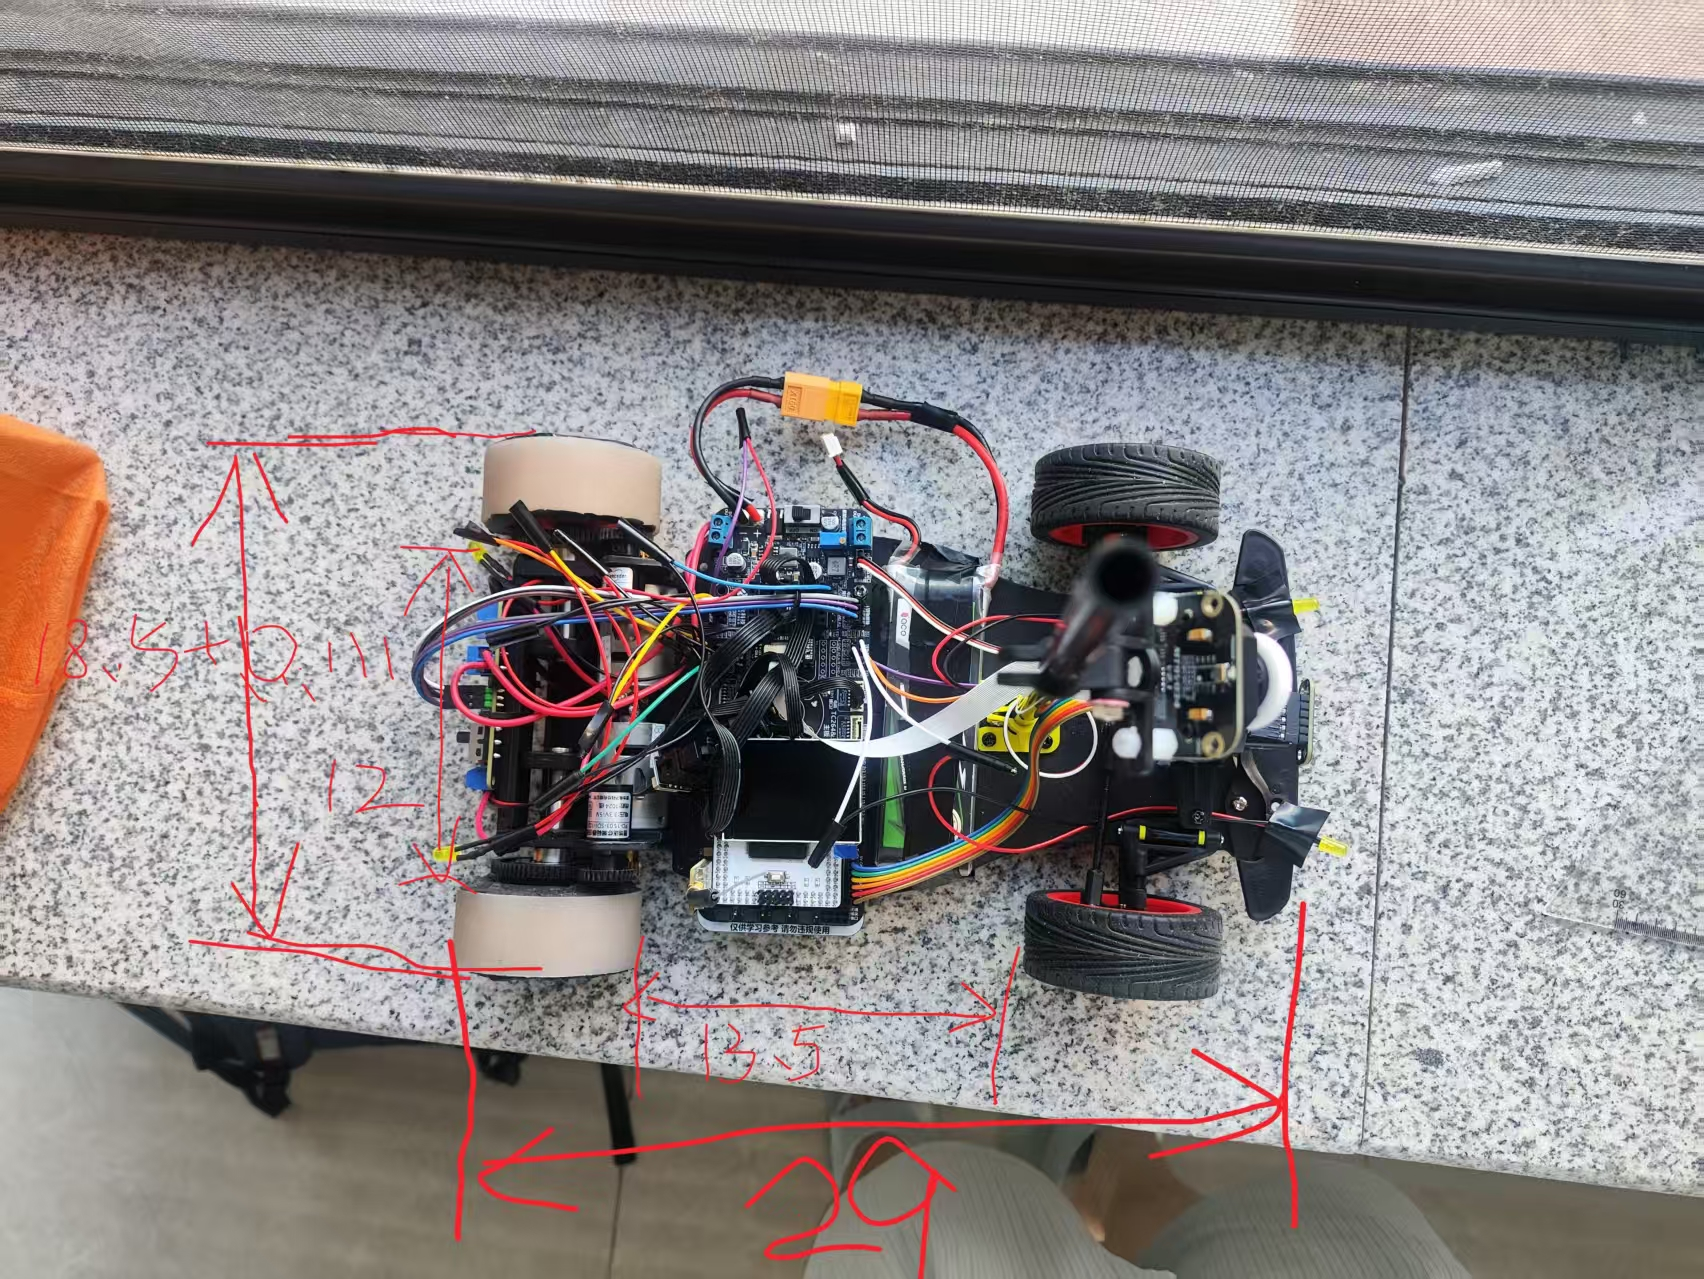
\includegraphics[width=0.68\textwidth]{MaiFigs/Mai俯视图.jpg}
  \caption{整车俯视布局与尺寸实测（单位：cm）}
  \label{fig:vehicle}
\end{figure}

\subsection{传感器安装}
摄像头通过竖直安装杆固定在车头正上方，镜头距地面约 25 cm，向下俯视赛道；光轴与水平面约成一定俯角，使画面近端覆盖车头前方约 0.3 m、远端覆盖约 1.5 m。镜头前加装飞思尔偏振片，用于抑制赛道反光，但会损失约 50\%~70\% 的进光量。摄像头安装支架需要保证左右水平，否则画面中的赛道中线会整体偏移，表现为车辆持续向一侧跑偏。DL1B 安装在车头前方，镜头朝前，用于检测挥手动作；其安装高度和角度需要避开地面反射和车头结构遮挡。车灯按左前、右前、左后、右后成对布置，刹车灯位于车尾，前大灯位于车头两侧。

\begin{figure}[htbp]
  \centering
  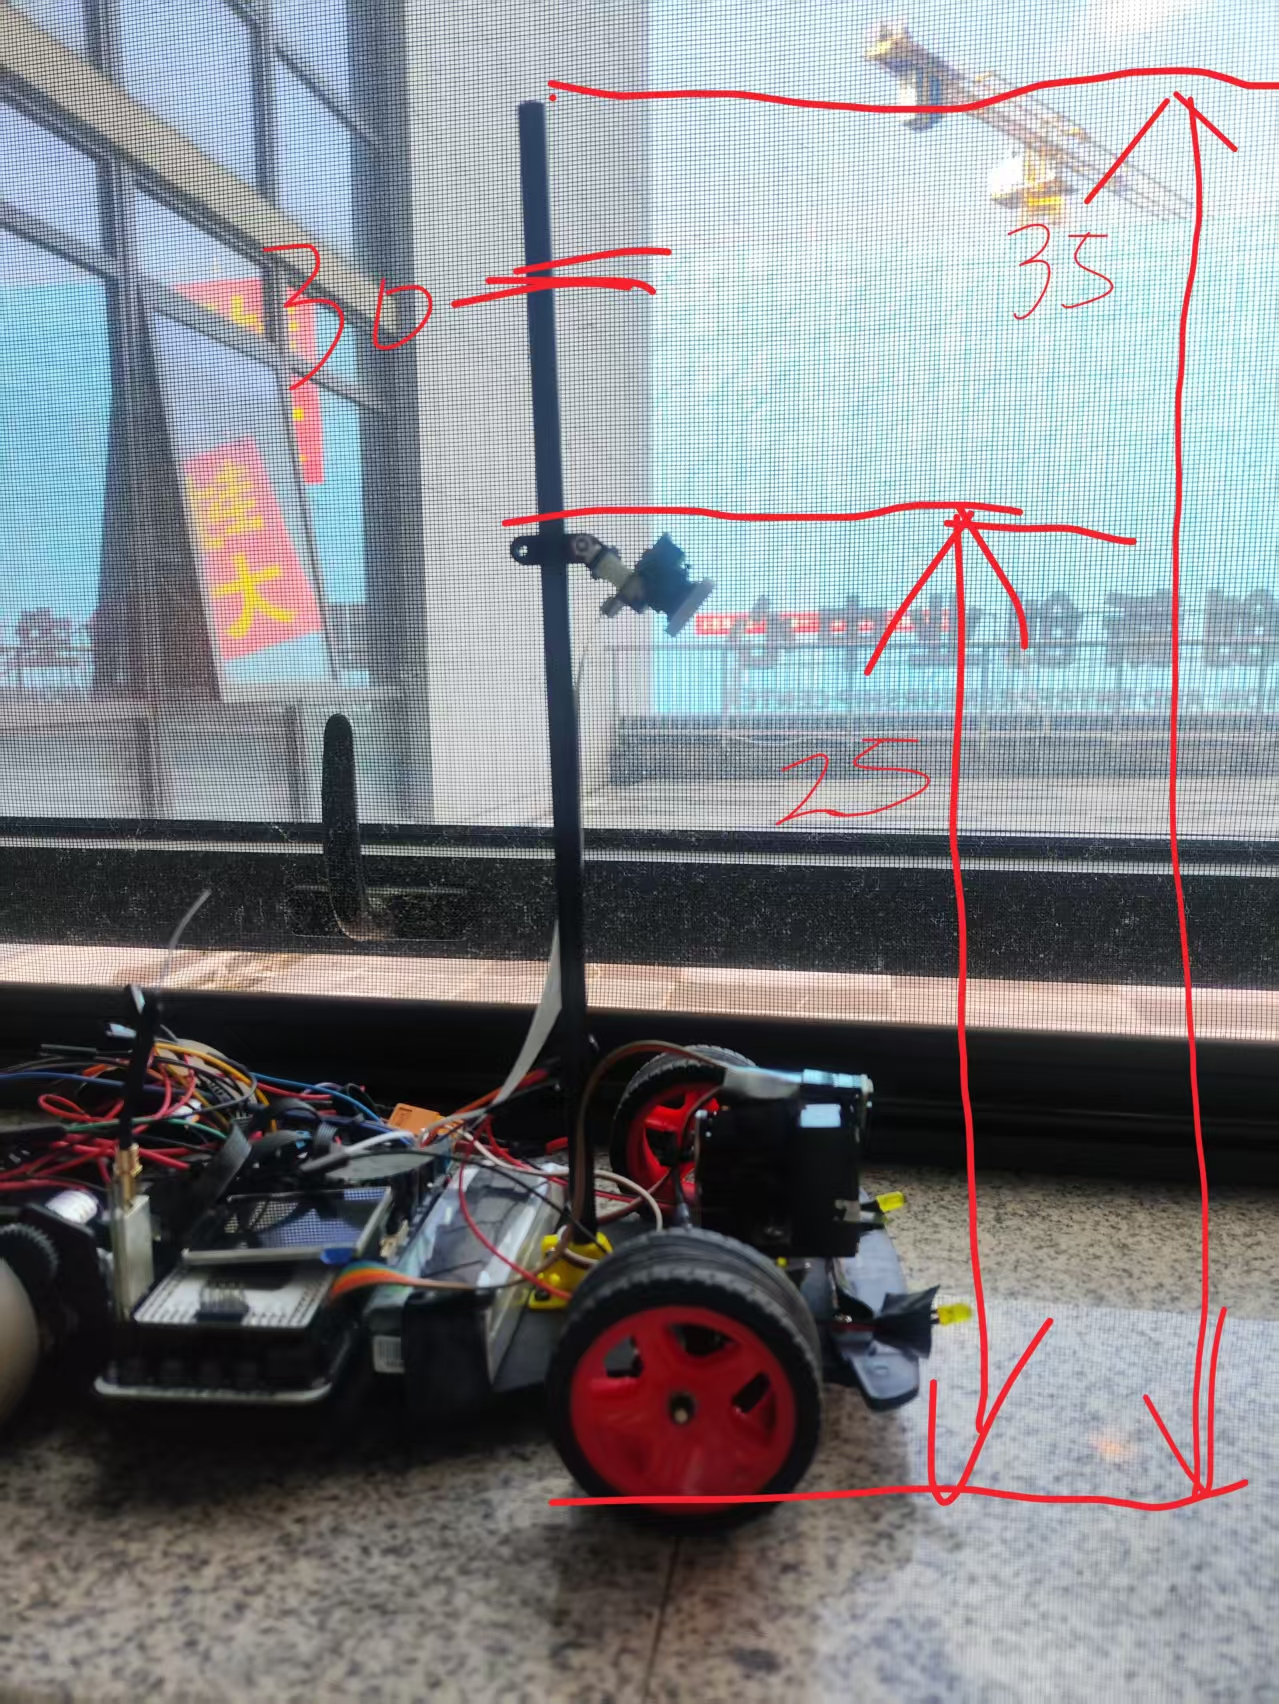
\includegraphics[width=0.40\textwidth]{MaiFigs/Mai高度.jpg}
  \caption{摄像头安装高度与改造前整车高度实测（单位：cm；杆体截短后整车约 25 cm）}
  \label{fig:sensors}
\end{figure}

\subsection{车灯布置与可维护性}
规则要求同侧前后转向灯同频率闪亮，恢复直行时熄灭；减速或停车时后刹车灯亮起；会车时前大灯闪烁 2$\sim$3 次。本文按“左 = 左前 + 左后”“右 = 右前 + 右后”成对控制，转向灯以约 130 ms 半周期闪烁。车灯驱动采用 GPIO 推挽输出，高电平点亮。

机械结构上，主控板、摄像头和 ToF 均通过插接件与排线连接，便于赛后拆装和更换。需要特别注意的是，部分灯引脚与 ToF 的软件 I\textsuperscript{2}C 引脚存在复用冲突，增加第二路 ToF 前必须先调整灯引脚；摄像头 FPC 排线需要固定，避免行驶振动导致接触不良。

\section{硬件设计}
\label{sec:hardware}

系统主要器件的选型与参数如表~\ref{tab:devices} 所示，后文按主控、感知、执行、通信和供电分别说明。

\begin{table}[htbp]
  \centering
  \caption{主要器件选型与参数}
  \label{tab:devices}
  \begin{tabular}{lll}
    \toprule
    器件 & 型号 / 规格 & 作用 \\
    \midrule
    主控 & Infineon TC264D，双核 200 MHz & 感知、决策与控制 \\
    核心板 & 仿逐飞 TC264 自制板 & 主控最小系统 \\
    主板 & 逐飞通用学习母板 V3.1 & 外设接口与供电分配 \\
    电机驱动 & 仿逐飞 DRV8701E 双路 H 桥 & 左右后轮驱动 \\
    车模 & 逐飞科技 C 车模 & 前轮转向、后轮双电机驱动 \\
    舵机 & SU400 & 前轮转向 \\
    编码器 & 普地 1024 线 mini，2 个 & 左右轮速度与里程 \\
    摄像头 & 总钻风 MT9V034 + 飞思尔偏振片 & 赛道与目标感知 \\
    测距 & DL1B（VL53L1X） & 非接触发车与前方测距 \\
    无线 & WIFI6B21-SPI V2.0 & 图传与 UDP 日志 \\
    显示 & IPS200 全彩屏（SPI） & 参数整定与状态监视 \\
    电池 & 格氏 ACE 3S 2200 mAh 30C & 11.1 V 动力电源 \\
    \bottomrule
  \end{tabular}
\end{table}

\subsection{主控与最小系统}
主控采用 Infineon AURIX TC264D 双核微控制器，主频 200 MHz，片内集成多路 PWM、正交编码器接口、SPI、I\textsuperscript{2}C、DMA 和定时器单元\upcite{tc26x}。选择该芯片的原因有三点：其一，双核结构可以把图像处理与控制任务分离，保证 5 ms 控制周期；其二，PWM、编码器和 DMA 资源丰富，可同时驱动舵机、双电机、摄像头和显示屏；其三，逐飞开源库提供了较完整的底层驱动\upcite{seekfree}，缩短了开发周期。

核心板为仿逐飞 TC264 自制板，主板为逐飞通用学习母板 V3.1，电机驱动板为仿逐飞 DRV8701E 自制双路 H 桥板。主板上集成电机驱动接口、舵机接口、摄像头接口、无线模块接口、IPS200 接口和按键。程序在 AURIX Development Studio 中编译，使用 TASKING 编译器生成 hex 文件，再通过 AURIX Flasher 烧录。

\subsection{视觉传感器}
视觉传感器采用总钻风 MT9V034 全局快门灰度摄像头\upcite{mt9v034}（底层驱动沿用 MT9V03X 库），配置分辨率为 120$\times$70。全局快门在曝光期间所有像素同时感光，避免了卷帘快门在高速运动下的果冻效应；灰度输出减少了数据量，使一帧图像仅 8400 字节，便于在微控制器上实时处理。摄像头通过并行数据线、VSYNC、PCLK 与 DMA 连接，CPU1 在帧完成标志置位后读取整帧。

摄像头的主要参数包括曝光时间和增益。曝光时间通过寄存器设置，增益通过全局增益寄存器设置。比赛中画面整体偏暗，最大灰度 $i_{\max}$ 只有约 120（满量程 255）。将曝光时间从 2300 增大到 10000，$i_{\max}$ 仅从 124 变到 122；将增益从 64 增大到 124，$i_{\max}$ 也仅从 124 变到 123，说明快门寄存器已受帧长限制、增益也已接近上限。进一步排查发现，镜头前的偏振片会造成约 50\%~70\% 的进光量损失，这是画面偏暗的主要原因。最终曝光时间设为 2300、增益设为 64，并在软件中保留在线调节接口；后续可通过摘除偏振片做对照实验，在反光抑制和进光量之间取舍。

\subsection{测距与发车检测}
发车检测采用 DL1B 激光测距模块\upcite{dl1b}（核心为 VL53L1X），通过软件 I\textsuperscript{2}C 与主控连接，SCL 为 P33\_4，SDA 为 P33\_5，从机地址为 0x29。DL1B 每次测距需要约 20$\sim$50 ms，驱动在“本轮尚未测完”时会返回 8192，因此 8192 不是故障码，而是“无有效新样本”的标志。早期代码把 8192 当作远距离或遮挡，导致上电自行发车；本文改为只消费“测量完成”标志置位后的新样本，从根源上排除了该问题。

软件 I\textsuperscript{2}C 的延时参数直接影响总线频率。驱动默认延时为 10，实测约 1.02 MHz，超过 DL1B 手册标称的 400 kHz；本文将其改为 50，实测约 448 kHz，既满足时序要求，又保留了足够的采样率。ToF 的 INT 引脚未启用，CPU1 采用轮询方式读取，避免中断引脚电平异常导致初始化失败。

\subsection{电机、舵机与编码器}
后轮采用两个有刷直流电机，由仿逐飞 DRV8701E 双路 H 桥板驱动，分别使用 PWM 和 DIR 信号。PWM 频率为 17 kHz，高于人耳可闻范围，可减少电机啸叫；DIR 信号控制正反转。左右电机分别使用普地 1024 线 mini 正交编码器（TIM6 和 TIM2 接口），编码器同轴安装在左右轮上，计数用于速度闭环和里程计算。实测编码器方向与电机方向相反，因此在软件中对左轮计数取负、右轮计数取正，两者必须同时修改，否则会出现飞车。

转向舵机为 SU400，采用 50 Hz PWM 控制，中位占空比实测为 917，行程为 $\pm$70 个占空比单位，约对应 $\pm$15$^\circ$。早期代码将上限写死为 915，而真实中位为 917，导致舵机无法向左打；本文改为运行时变量 \texttt{Steer\_Mid}，并让上下限随中位变化，解决了单方向转向问题。

\subsection{无线通信与人机接口}
无线模块为 WIFI6B21-SPI V2.0，属于调试设备，比赛时可拆下；它通过 SPI3 与主控连接，SCK 为 P22\_3，MOSI 为 P22\_0，MISO 为 P22\_1，CS 为 P22\_2。模块的 INT 引脚在本板上恒为低电平，原版驱动等待 INT 会永久超时；本文将驱动改为固定延时，普通命令延时 250 ms、连接 WiFi 延时 3 s、连接 TCP 延时 1.5 s。代价是上电后约 15 s 屏幕才亮，这段时间黑屏属于正常现象。

无线模块支持 TCP 和 UDP 两种模式。比赛调试阶段使用 UDP 向电脑回传日志，每 10 个主循环发送一行，约 250 ms 一行；需要看图时切换为 TCP，通过逐飞助手接收灰度图或二值图。SPI 时钟从 30 MHz 降到 10 MHz，以提高长排线连接的稳定性。

人机接口包括 IPS200 全彩屏（SPI 版，调试设备，比赛时可拆）和 5 个按键接口（S1$\sim$S5，当前主要使用 S2$\sim$S5）。屏幕分为 3 页：page1 显示图像、边界、锥桶和识别结果；page2 显示电机、编码器和速度；page3 显示 15 个可调参数、WiFi 诊断和 ToF 状态。按键 S2 翻页，S5 切换参数，S3/S4 减小/增大参数，长按 S5 保存到 flash。

\subsection{电源与车灯}
整车由格氏 ACE 系列 3S 2200 mAh 30C 锂聚合物电池供电，标称电压 11.1 V。主控板、摄像头、ToF、WiFi 模块和屏幕由板上稳压电路供电；电机和舵机由电池直接供电。车灯共 8 路，全部为高电平点亮，其中左前转向 P02\_4、右前转向 P02\_5、左后转向 P02\_6、右后转向 P02\_7、左后刹车 P20\_11、右后刹车 P00\_8、左前大灯 P20\_13、右前大灯 P20\_14。前大灯引脚尚待最终确认，目前借用刹车灯附近引脚。

\subsection{引脚分配与硬件问题}
关键引脚分配见附录 B 表 B.1。正文只列出最容易出问题的几组：舵机 PWM 为 P33\_9；右轮 PWM/DIR 为 P21\_2/P21\_3，编码器为 P20\_3/P20\_0；左轮 PWM/DIR 为 P21\_4/P21\_5，编码器为 P33\_7/P33\_6；摄像头数据为 P00\_0$\sim$P00\_7；ToF 软件 I\textsuperscript{2}C 为 P33\_4/P33\_5；WiFi SPI 为 P22\_0$\sim$P22\_3。完整表格放在附录，便于硬件维护时查阅。

硬件调试中遇到的主要问题如下：
\begin{enumerate}
  \item \textbf{WiFi INT 引脚恒低}：模块 INT 始终为低，驱动等待中断会超时，改为固定延时后解决；
  \item \textbf{DL1B I\textsuperscript{2}C 超频}：默认延时对应约 1.02 MHz，超过 400 kHz 上限，改为延时 50 后稳定；
  \item \textbf{编码器与 GPIO 复用}：P33\_7/P33\_6 是左轮编码器输入，不能当作普通 GPIO 使用，否则速度反馈恒为 0，PWM 顶满导致飞车；
  \item \textbf{车灯与 ToF 引脚冲突}：P20\_11/P20\_14 与第二路 ToF 的软件 I\textsuperscript{2}C 冲突，增加第二路 ToF 前必须换脚；
  \item \textbf{断言静默停机}：坐标越界等断言失败会关闭 PWM、PIT 和外部中断，表现为屏幕仍刷新但电机不转，需要检查屏幕坐标和 flash 页号。
\end{enumerate}

\section{软件设计}
\label{sec:software}

\subsection{软件总体架构}
软件采用“前后台 + 中断”的结构。CPU0 主循环负责按键、屏幕和日志；5 ms 定时中断负责速度环和转向环；10 ms 定时中断负责车灯和 ToF 判定。CPU1 主循环等待摄像头帧完成标志，依次执行阈值计算、二值化、边界提取、标线识别、锥桶识别、反光抑制和目标点计算，如图~\ref{fig:pipeline} 所示。

\begin{figure}[htbp]
  \centering
  \begin{tikzpicture}[
    node distance=4mm and 4mm,
    box/.style={draw,rounded corners,minimum width=3.35cm,minimum height=0.7cm,align=center,font=\zihao{-5}},
    arr/.style={-{Latex[length=2mm]},thick}]
    \node[box] (a) {帧完成标志};
    \node[box,right=of a] (b) {迭代阈值};
    \node[box,right=of b] (c) {二值化};
    \node[box,right=of c] (d) {边界 / 补线};
    \node[box,below=of d] (e) {中线拟合};
    \node[box,left=of e] (f) {标线识别};
    \node[box,left=of f] (g) {锥桶识别};
    \node[box,left=of g] (h) {反光抑制 / 目标点};
    \draw[arr] (a) -- (b); \draw[arr] (b) -- (c); \draw[arr] (c) -- (d);
    \draw[arr] (d) -- (e);
    \draw[arr] (e) -- (f); \draw[arr] (f) -- (g); \draw[arr] (g) -- (h);
  \end{tikzpicture}
  \caption{CPU1 图像处理流程}
  \label{fig:pipeline}
\end{figure}

各模块之间通过全局数组和标志变量传递数据：\texttt{Left\_Line[61]}、\texttt{Right\_Line[61]}、\texttt{Mid\_Line[61]} 保存逐行边界和中线，\texttt{Width\_Real[61]} 保存宽度，\texttt{Result\_Far\_Row} 保存本帧最远可信行，\texttt{cone\_cnt}、\texttt{cone\_x}、\texttt{mk\_cw\_seen}、\texttt{mk\_dia\_seen} 等保存识别结果。控制层只读取这些结果，不直接访问图像，降低了模块耦合。

\subsection{图像预处理与自适应阈值}
摄像头输出 120$\times$70 的 8 位灰度图，灰度范围 0$\sim$255。赛道为黑色，标线和锥形标为白色或浅色，理论上用固定阈值即可分割；但现场光照变化、镜头暗角和地面反光会使同一阈值在不同区域产生完全不同的结果。为此本文采用迭代直方图分割法\upcite{otsu1979}：

\begin{enumerate}
  \item 统计整帧 256 级灰度直方图，求最小灰度 $g_{\min}$ 和最大灰度 $g_{\max}$；
  \item 取初始阈值 $T_0=(g_{\min}+g_{\max})/2$；
  \item 分别计算 $[g_{\min},T_0)$ 和 $(T_0,g_{\max}]$ 两部分的灰度均值 $A_1$、$A_2$，令 $T_0=(A_1+A_2)/2$；
  \item 重复步骤 3，直到 $T_0$ 不再变化或达到 200 次迭代；
  \item 按式~\eqref{eq:threshold} 对阈值进行比例缩放并限幅。
\end{enumerate}

\begin{equation}
  T=\mathrm{clamp}\left(T_0\cdot\frac{z_y+d}{100},\ 12,\ 240\right)
  \label{eq:threshold}
\end{equation}

其中 $z_y$ 为阈值系数，默认 95；$d$ 为阈值偏置，默认 0。系数大于 100 时判为白色的像素减少，小于 100 时增多。限幅 12$\sim$240 保证不会出现全白或全黑。二值化时，灰度大于 $T$ 的像素置 255，否则置 0。

实际调试发现，画面平均灰度 $i_{\mathrm{avg}}$ 在正常黑赛道上只有 3$\sim$8，而早期锥桶识别沿用了“平均灰度小于 10 就放弃”的保护，导致约 79\% 的帧被误丢弃。本文删除了该保护，仅保留“平均灰度大于 190 视为过曝”的判断。这个例子说明，图像算法的保护条件必须结合具体场景，不能盲目复用。

\subsection{赛道边界提取与中线拟合}
边界提取从画面最下方一行（第 59 行）开始，逐行向上处理。第一行需要特殊处理：如果第 59 行中点像素为黑，说明车辆可能偏出赛道或处于赛道边缘，此时分别从左、右两侧扫描，选择赛道宽度较大的一侧作为初始边界；否则以画面中心为起点向两侧扫描。

从第二行开始，以上一行的中线 \texttt{Mid\_Line[i+1]} 为起点，向左右各寻找第一处“黑转白”跳变，分别作为本行的左右边界。若某一侧没有找到跳变，则标记该侧需要补线；补线采用上一行边界或已拟合直线的斜率进行线性外推。每处理完一行，计算宽度 \texttt{Width\_Real[i]=Right\_Line[i]-Left\_Line[i]}，并在宽度突增超过 10 px 或边界跳变超过 10 px 时置补线标志。

中线拟合采用最小二乘法。对第 58 行到 \texttt{Line\_Count+2} 行的中线点 $(i,\ \mathrm{Mid\_Line}[i])$ 拟合直线 $x=ka\cdot i+kb$，再外推到第 20 行，得到目标点：
\begin{equation}
  P = \mathrm{clamp}\left(ka\cdot 20+kb,\ 2,\ 118\right)
  \label{eq:point}
\end{equation}
选择第 20 行而不是最近的第 59 行，是因为远端目标点具有前视作用，可以让车辆提前转向，减少近端抖动对舵机的影响。拟合行数不足时，\texttt{Result\_Far\_Row} 会变小，控制层据此判断本帧是否可信。

\subsection{双车道宽度归一化与迟滞选道}
双车道赛道的特殊之处在于：车道中线是虚线，虚线有白色线段，也有断口。边界提取从画面中心向两侧寻找“第一处白色跳变”，因此同一帧的检测结果会出现两种完全不同的情况：
\begin{enumerate}
  \item 虚线当前行有白色线段：扫描到“左实线 + 虚线”，宽度约 43 px，对应一条车道；
  \item 虚线当前行是断口：虚线被跳过，扫描到“左实线 + 右实线”，宽度约 90$\sim$116 px，对应整条路。
\end{enumerate}

原算法用同一个公式 $P_t=L+W\cdot k/100$ 计算目标点，其中 $k$ 为选道系数。当 $W=43$ 时，$P_t$ 已经贴到右边缘之外；当 $W=116$ 时，$P_t$ 才是右道中心。同一个 $k$ 在两种宽度下算出的根本不是同一个位置，车辆就会在左右道之间来回穿梭。日志统计显示，729 帧中 $R=117$（扫描到边界仍未找到线）出现 173 次，占 24\%；$W$ 呈双峰分布，30$\sim$49 px 有 40 帧，80$\sim$119 px 有 27 帧。

本文提出宽度归一化：先判断当前扫到的是一条道还是整条路，再分别计算目标点。设左右边界为 $L$、$R$，宽度 $W=R-L$，单道宽度的兜底值为 $W_0=43$，则
\begin{equation}
  P_t=
  \begin{cases}
    L+W/2, & W\le 70,\\[2pt]
    L+W/4, & W>70,\ k\le 50,\\[2pt]
    L+3W/4, & W>70,\ k>50.
  \end{cases}
  \label{eq:target}
\end{equation}
其中 $k\le 50$ 表示选择左道，$k>50$ 表示选择右道。$W\le 70$ 时车辆待在自己所在的车道中心；$W>70$ 时按选道系数取左道或右道中心。

由于 $W$ 是连续变化的，70 px 这条分界线正好切在单道与整条路的中间，抖动一下就会在两种算法之间切换，实测相邻目标点最大跳变 92 px。为此本文加入迟滞：
\begin{equation}
  \text{mode}=
  \begin{cases}
    1\ (\text{整条路}), & W>85,\\
    0\ (\text{单道}), & W<60,\\
    \text{保持不变}, & 60\le W\le 85.
  \end{cases}
  \label{eq:hysteresis}
\end{equation}
只有 $W>85$ 才进入整条路模式，$W<60$ 才回到单道模式，中间 60$\sim$85 px 保持上一次判断，从而避免模式抖动。

单边丢线时，用学到的单道宽度 $W_{\mathrm{ema}}$ 向缺失一侧补半个或一个半道宽：
\begin{equation}
  P_t=
  \begin{cases}
    L+\dfrac{W_{\mathrm{ema}}}{2}, & \text{仅左边界，选左道},\\[6pt]
    L+\dfrac{3W_{\mathrm{ema}}}{2}, & \text{仅左边界，选右道},\\[6pt]
    R-\dfrac{W_{\mathrm{ema}}}{2}, & \text{仅右边界，选右道},\\[6pt]
    R-\dfrac{3W_{\mathrm{ema}}}{2}, & \text{仅右边界，选左道}.
  \end{cases}
  \label{eq:single}
\end{equation}
$W_{\mathrm{ema}}$ 只学习 $W\le 70$ 的单道样本，避免被整条路的 116 px 污染。

为了防止单边补线把目标点推到画面外，本文还加入位置合理性检查和限幅：左边界必须位于画面左侧 3/4 内，右边界必须位于右侧 3/4 内；目标点限制在画面中心 $\pm$45 px 内，锥桶区域收紧到 $\pm$25 px。实测曾出现 $L=100$、$R=117$、$W=17$ 的异常帧，单边补线算出 $P_t=127$（画面只有 0$\sim$119），舵机从满左直接甩到满右；限幅后该问题消失。

\subsection{不可信帧保持}
人行横道、斑马线和强反光会让整幅画面变白，边界提取随即失效：中线拟合可能塌到画面最左边（$P\le 6$）或最右边（$P\ge W-6$），可信行数骤减，目标点跳到画面外。早期代码虽然计算了 \texttt{steer\_guard\_bits}，但没有真正使用，舵机仍然拿垃圾数据打方向。日志中横道前出现过 $P_t$ 从 57 跳到 86、占空比从 934 掉到 863 的情况，表现为车头突然右偏。

本文把保护位真正接入控制：当目标点越界，或 \texttt{steer\_guard\_bits} 的 0x0004（中线贴左）、0x0008（中线贴右）、0x1000（可信行不足）任一置位时，判定本帧不可信，沿用上一次可信目标点 \texttt{pt\_good}；连续 2 s（400 个 5 ms 周期）都不可信时，才回到画面中心。这样既避免了单帧垃圾数据打方向，又能在真正丢线时让车辆回中，避免一直保持错误方向。

保护位还包括宽度过窄/过宽、左右边界撞墙、起跑后 1 s 图像稳定期等。所有保护位集中在一个 16 位变量中，便于日志观察和问题定位。图~\ref{fig:width} 给出了宽度跳变与迟滞选道的示意。

\begin{figure}[htbp]
  \centering
  \begin{tikzpicture}[scale=0.92,transform shape,font=\zihao{5}]
    % 左图：单道
    \draw[thick] (0,0) rectangle (6,3.2);
    \draw[thick] (0,1.6) -- (6,1.6);
    \draw[dashed,thick] (3,0) -- (3,3.2);
    \node at (1.5,0.8) {左道};
    \node at (4.5,0.8) {右道};
    \draw[<->] (0,2.45) -- (3,2.45) node[midway,above] {$W\approx43$ px};
    % 右图：整条路
    \begin{scope}[xshift=8cm]
      \draw[thick] (0,0) rectangle (6,3.2);
      \draw[thick] (0,1.6) -- (2.2,1.6);
      \draw[thick] (3.8,1.6) -- (6,1.6);
      \draw[dashed,thick] (3,0) -- (3,1.6);
      \draw[dashed,thick] (3,1.6) -- (3,3.2);
      \node at (1.5,0.8) {左道};
      \node at (4.5,0.8) {右道};
      \draw[<->] (0,2.45) -- (6,2.45) node[midway,above] {$W\approx90\sim116$ px};
    \end{scope}
    \node at (3,-0.6) {(a) 虚线当前行有白段};
    \node at (11,-0.6) {(b) 虚线当前行是断口};
  \end{tikzpicture}
  \caption{虚线断口导致的赛道宽度跳变}
  \label{fig:width}
\end{figure}

\subsection{转向控制}
转向控制采用变增益位置式 PD。设目标点为 $P_t$，画面中心为 $P_0=60$，误差 $e=P_t-P_0$，则
\begin{equation}
  \begin{aligned}
    K_p &= 0.2\,|e|,\\
    K_d &= 1.6K_p,\\
    u &= K_p e + K_d\,(e-e_{\mathrm{last}}),\\
    \delta &= \delta_{\mathrm{mid}}-u+\delta_{\mathrm{trim}},
  \end{aligned}
  \label{eq:pd}
\end{equation}
其中 $\delta$ 为舵机占空比，$\delta_{\mathrm{mid}}=917$，$\delta_{\mathrm{trim}}$ 为转向微调。误差越大，$K_p$ 越大，转向越猛；误差越小，$K_p$ 越小，转向越柔和。这种变增益设计使车辆在大偏差时快速回中，在小偏差时避免高频抖动。微分项抑制误差变化率，减少超调。

转向输出经过两级限幅：先限制在 $[\delta_{\mathrm{mid}}-70,\ \delta_{\mathrm{mid}}+70]$，再叠加微调后再次限幅，保证舵机不会堵转。发车后的短暂稳定期内，摄像头曝光尚未稳定，转向保持中位；稳定后进入闭环。未发车时，控制层仍然计算并显示目标点，但不驱动舵机，便于现场检查图像算法是否正常。

\subsection{速度控制}
速度环采用增量式 PID。设目标速度为 $v_{\mathrm{ref}}$，编码器反馈速度为 $v$，误差 $e_k=v_{\mathrm{ref}}-v$，则
\begin{equation}
  \Delta u=K_p(e_k-e_{k-1})+K_i e_k+K_d(e_k-2e_{k-1}+e_{k-2}),
  \label{eq:pid}
\end{equation}
输出 $u_k=u_{k-1}+\Delta u$，并限制在 $\pm3000$ 内。参数取 $K_p=40$、$K_i=6$、$K_d=1$。原参数按高速工况整定，低速时积分过强，容易抖动；降低 $K_i$ 后低速稳定性明显改善。

基础目标速度为 210，乘以速度百分比 12\% 后约为 25。为了抑制起步冲击，加入软起动：每 40 个 5 ms 周期（200 ms）目标速度增加 1，从 0 加速到 25 约需 5 s。减速和停车不做缓降，保证随时能停。电机 PWM 频率 17 kHz，输出前做绝对值限幅 $\pm3000$，这是最后一道软件保险：即使 PID 失控或方向接反，电机输出也不会超过设定值。

编码器同时用于里程估计。每个计数对应约 0.0288 cm，车辆前进时累计 \texttt{Run\_Odo}，后退或静止不累计。里程用于标定“看到标线时车头距离标线多远”，以及状态机中的 60 cm 恢复距离。

\subsection{锥形标识别与锁存绕行}
红色锥形标在灰度图中的灰度约为 76，而二值阈值约为 48，因此锥形标整体变白，与车道线颜色相同。颜色无法区分，只能利用宽度：车道线宽约 2 cm，对应 2$\sim$3 px；锥形标白环宽约 1 cm，但锥体本身宽 6$\sim$9 cm，对应 5$\sim$40 px。本文据此设计锥形标检测：

\begin{enumerate}
  \item 在图像第 14$\sim$56 行、第 6$\sim$111 列范围内逐行扫描白段；
  \item 若左右边界看起来可信（左边界在左半幅、右边界在右半幅、宽度大于 25 px），只扫描车道内部，避免把赛道外的白色地板当成锥桶；
  \item 记录每个白段的起点、宽度和中心 $x$，宽度在 5$\sim$40 px 的白段作为候选；
  \item 将当前行的候选与上一行、横向偏差不超过 10 px 的 blob 合并，形成二维 blob；
  \item 统计有效 blob 数 $N$，并计算近端（行号不小于 36）blob 的平均 $x$ 作为 \texttt{cone\_x}；近端没有时退回全体平均；
  \item 当 $N\ge2$ 时置 \texttt{cone\_ok}=1。
\end{enumerate}

早期版本要求 blob 至少占 2 行，但锥形标白环只有约 1 cm 高，二值化后往往只有 1 行，导致大量漏检；改为至少 1 行后，锥桶计数从 1$\sim$2 增加到 6$\sim$11。另一个问题是 \texttt{cone\_x} 取“最靠下的 blob”，而白环是碎片化的，相邻帧可能在 61、102、79、37 之间跳动，导致绕行方向反复变化；改为近端 blob 平均后，方向判断稳定得多。

绕行决策采用锁存式状态机，如图~\ref{fig:cone} 所示。第一次满足 \texttt{cone\_ok} 且 $N\ge2$ 时，比较锥桶左右两侧的剩余空间：
\begin{equation}
  \mathrm{dir}=
  \begin{cases}
    +1, & R_{\mathrm{room}}>L_{\mathrm{room}},\\
    -1, & R_{\mathrm{room}}\le L_{\mathrm{room}},
  \end{cases}
  \label{eq:cone_dir}
\end{equation}
其中 $L_{\mathrm{room}}=\texttt{cone\_x}-L$，$R_{\mathrm{room}}=R-\texttt{cone\_x}$。边界不可信时，改为按锥桶位于画面中心左侧还是右侧决定方向。确定方向后，锁存 200 个 5 ms 周期（1 s），期间目标点固定为 $P_0+\mathrm{dir}\times22$，不再根据误差持续修正。1 s 后解除锁存，回到循迹；锥桶连续 1 s 看不见后，才允许下一组锥桶触发新的变道。

\begin{figure}[htbp]
  \centering
  \begin{tikzpicture}[
    node distance=5mm,
    box/.style={draw,rounded corners,minimum width=3.4cm,minimum height=0.8cm,align=center,font=\zihao{5}},
    arr/.style={-{Latex[length=2mm]},thick}]
    \node[box] (see) {看到锥桶\\$N\ge2$};
    \node[box,right=of see] (dir) {比较左右空间\\确定变道方向};
    \node[box,right=of dir] (hold) {锁存 1 s\\目标点 $P_0\pm22$};
    \node[box,below=of hold] (back) {解除锁存\\回到循迹};
    \node[box,below=of dir] (clear) {锥桶离开 1 s\\允许下一组};
    \draw[arr] (see) -- (dir);
    \draw[arr] (dir) -- (hold);
    \draw[arr] (hold) -- (back);
    \draw[arr] (back) -- (clear);
  \end{tikzpicture}
  \caption{锥形标锁存绕行流程}
  \label{fig:cone}
\end{figure}

这里有一个重要的控制经验：变道的量只能靠时间，不能靠误差。因为检测到的车道是跟着车走的：车往左挪，车道在画面里也往左挪，目标点与画面中心的误差重新出现，控制器就会一直往左打。实测中曾出现连续左满舵 8 次、越转越左；改为固定 1 s 锁存后，一次只变一道，行为可预测。当前方案仍是近似方案，锥形标实际是一组斜跨两条道的斜线，更精确的做法是把所有 blob 拟合为直线 $x=a\cdot row+b$，让车辆沿斜线平行行驶。

\subsection{道路标线识别与停车状态机}
道路标线识别在图像中央竖带（第 36$\sim$84 列、第 8$\sim$58 行）内进行。对每一行统计白点数、最长连续白段和细白段数量，按以下规则分类：
\begin{enumerate}
  \item \textbf{人行横道}：最长连续白段不小于 22 px，且白点数不少于 22，连续出现至少 4 行；
  \item \textbf{减速菱形}：同一行至少有 2 条宽度 2$\sim$10 px 的细白段，且白点数不超过 50，连续出现 6$\sim$40 行；
  \item \textbf{停车线}：近车头（行号大于 52）出现 1$\sim$3 行横道式白带。
\end{enumerate}
人行横道是横跨车道的连续白带，菱形是两条斜边夹一条中线，停车线是一条靠近车头的单白带，三者在行宽、白点数和连续行数上都有区别。整幅过曝（平均灰度大于 190）或过暗（小于 10）时，标线识别直接返回，避免起跑瞬间的过曝误报。

标线状态机如图~\ref{fig:marker} 所示。状态 0 为空闲；连续 8 帧看到菱形后进入状态 1（慢行）；状态 1 中，连续 15 帧看到人行横道且近端行号不小于 45 时进入状态 2（停车计时）；停车 1000 个 5 ms 周期（5 s）后进入状态 3（已通过）；人行横道消失后回到状态 0。菱形消失且前进里程超过 60 cm 时，也从状态 1 回到状态 0，恢复原速。

\begin{figure}[htbp]
  \centering
  \begin{tikzpicture}[
    node distance=1.4cm,
    st/.style={draw,circle,minimum size=1.5cm,align=center,font=\zihao{5}},
    arr/.style={-{Latex[length=2mm]},thick}]
    \node[st] (s0) {0\\空闲};
    \node[st,right=of s0] (s1) {1\\慢行};
    \node[st,right=of s1] (s2) {2\\停车};
    \node[st,right=of s2] (s3) {3\\通过};
    \draw[arr] (s0) -- node[above,font=\zihao{6}]{菱形 8 帧} (s1);
    \draw[arr] (s1) -- node[above,font=\zihao{6}]{横道 15 帧} (s2);
    \draw[arr] (s2) -- node[above,font=\zihao{6}]{5 s} (s3);
    \draw[arr] (s3) to[bend left=35] node[below,font=\zihao{6}]{横道消失} (s0);
    \draw[arr] (s1) to[bend right=35] node[below,font=\zihao{6}]{菱形消失且前进 60 cm} (s0);
  \end{tikzpicture}
  \caption{道路标线状态机}
  \label{fig:marker}
\end{figure}

状态 1 中速度降为原速的 50\%，状态 2 中电机输出 0，车辆自然滑停。刹车灯在状态 1 和状态 2 亮起，满足规则“减速或停车时后刹车灯亮起”的要求。当前实现是“进入状态 1 直接降一半”，还不是规则要求的“逐渐减速”；后续可以按里程或时间分 3$\sim$5 档逐级降速，避免扣分。

\subsection{非接触发车}
非接触发车由 CPU1 和 CPU0 协作完成。CPU1 轮询 DL1B，只有当“测量完成”标志置位时，才把距离写入 \texttt{tof\_sample\_mm} 并置 \texttt{tof\_new\_sample}=1；CPU0 的 10 ms 中断消费该标志，保证每个测量样本只统计一次，8192 无效值不会冲掉有效样本。

判定逻辑如下：
\begin{enumerate}
  \item 若连续 1 s 没有收到任何有效样本，认为前方空旷，置布防标志 \texttt{tf\_armed}=1；
  \item 布防后，维护最近 12 个有效样本的滑动窗口，统计其中距离在 10$\sim$500 mm 的样本数；
  \item 若窗口已填满且命中数不少于 8，置位 \texttt{start\_trigger}=1；
  \item 命中条件为 $10\le d<500$ mm；车停在墙边时一开始就读到近距，无法布防，因此不会抢跑。
\end{enumerate}

布防需要前方至少 1 s 没有有效近距样本；布防后挥手，约 0.4$\sim$0.5 s 内累计 8 次命中即发车，满足非接触发车要求。屏幕 page3 最后一行显示 \texttt{To（当前距离）A（是否布防）H（命中数）}，便于现场判断：\texttt{A=0} 表示还没布防，\texttt{A=1} 可以挥手，\texttt{H} 从 0 涨到 8 即发车。

\subsection{调试与参数管理}
系统提供 5 个可在线整定的参数，如表~\ref{tab:params} 所示。参数保存在 flash 第 11 页，备份页为第 10 页；上电时先检查有效标记，再逐项校验范围，不合法则退回代码默认值。早期版本曾把备份页写成 17，而驱动只支持 0$\sim$11 页，触发断言后 PWM、PIT 和外部中断全部关闭，表现为屏幕仍刷新但车不动。改为第 10 页后问题解决。

\begin{table}[htbp]
  \centering
  \caption{在线整定参数}
  \label{tab:params}
  \begin{tabular}{llll}
    \toprule
    参数 & 作用 & 默认值 & 范围 \\
    \midrule
    \texttt{zyuzhi} & 二值化阈值系数 & 95 & 20$\sim$255 \\
    \texttt{Differ} & 阈值偏置 & 0 & $-50\sim50$ \\
    曝光时间 & 摄像头曝光 & 2300 & 60$\sim$10000 \\
    增益 & 摄像头模拟增益 & 64 & 16$\sim$124 \\
    \texttt{STrim} & 转向微调 & 16 & $-60\sim60$ \\
    \bottomrule
  \end{tabular}
\end{table}

调参阶段将 \texttt{PARAM\_TUNING} 置 1，上电不读 flash，一律使用代码默认值，避免旧参数覆盖新默认；转向中位是例外，上电仍从第 10 页恢复，保证现场校准结果不丢失。长按 S5 保存参数，长按 S3 恢复默认，长按 S4 切换图传内容。

UDP 日志每 10 个主循环发送一行，包含 30 余个字段：帧号、目标点、扫描行号、可信行、左右边界、宽度、舵机占空比、状态机、阈值、ToF 距离、曝光、增益、图像最小/最大/平均灰度、标线结果、锥桶计数、里程、保护位等。电脑端运行 \texttt{car\_log.py} 接收并按行打印，可以离线分析宽度分布、目标点跳变和发车时序。

\subsection{赛项一：超车与会车决策}
\label{sec:overtake}

赛项一与赛项二共用底盘、摄像头、执行机构和调试系统，但使用两套独立工程：赛项二代码在 \texttt{bizhang\_1108}，赛项一代码在 \texttt{chaoche2024\_1109}。赛项一工程沿用同一套灰度图像、边界提取、中线拟合以及转向/速度控制思路，新增 \texttt{Car\_Scan()} 前方车辆检测和 \texttt{Overtake\_Control()} 行为状态机。代码用 \texttt{OVERTAKE\_ENABLE} 作为总开关，默认值为 0；关闭时状态机只做复位，不改舵机和车灯，避免未标定的参数影响正常行驶。

\subsubsection{基于车道半区白点占比的车辆检测}
赛项一的前车是 1:8$\sim$1:15 遥控车。赛道宽 1.5 m、单车道 45 cm，在 120$\times$70 图像中一条车道约 58 px，一辆车约 26$\sim$38 px 宽，且位于本车道内部；这与只有 2$\sim$3 px 宽的车道线有明显区别。难点在于车壳颜色未知：浅色车壳在二值图中是白的，深色车壳与黑色赛道一样是黑的，无法用固定颜色阈值识别。

本文不直接“识别车”，而是统计两条边线之间左、右半车道的白点占比。对第 22$\sim$54 行逐行处理：先取该行左右边界的中点，再把中线左侧（左边界加 3 px 到中点减 5 px）和右侧（中点加 5 px 到右边界减 3 px）分别作为左右半车道；只有边界可信、中点位于 25$\sim$95 px、单行有效列数不少于 8 时才统计。分别累计左右半车道的白点数与总列数，得到整帧占比
\begin{equation}
  p_{\mathrm{L}}=\frac{N_{\mathrm{white,L}}}{N_{\mathrm{total,L}}}\times100\%,\qquad
  p_{\mathrm{R}}=\frac{N_{\mathrm{white,R}}}{N_{\mathrm{total,R}}}\times100\%.
  \label{eq:car_pct}
\end{equation}
同时记录单行白点占比超过 45\% 的最靠下那一行，作为“车离车头多近”的粗略度量。输出量为 \texttt{car\_pct\_l}、\texttt{car\_pct\_r}、\texttt{car\_row\_l}、\texttt{car\_row\_r}，并显示在 IPS200 的 page3 上，便于现场调阈值。

正常赛道上两条边线之间只有一条细虚线，左右半车道白点占比都较低；浅色车进入某一半车道时，该半区占比会明显升高。设车辆靠右行驶（\texttt{OVT\_OWN\_RIGHT=1}），则右半区对应本车道前车，左半区对应对向车。当前判据为：本车道白点占比不小于 45\%，且最近行号不小于 40，认为前方有同向车；对向半区占比不小于 45\%，认为有对向车。

\subsubsection{超车与会车状态机}
超车状态机如图~\ref{fig:overtake} 所示，分为 IDLE、GO、BACK 三态。IDLE 下，若本车道连续 20 个 5 ms 周期（100 ms）检测到前车且不在冷却期，进入 GO；GO 把转向参考点向左平移 25 px，同时点亮左转向灯，保持 400 个周期（2 s）；随后进入 BACK，参考点回到本道中心，点亮右转向灯，保持 300 个周期（1.5 s）；BACK 结束后回到 IDLE，并进入 300 个周期（1.5 s）冷却，避免同一辆车反复触发。参考点的平移量 \texttt{ovt\_offset} 直接叠加到 PD 控制器的目标中心上，正值对应向左借道。

\begin{figure}[htbp]
  \centering
  \begin{tikzpicture}[
    node distance=1.3cm,
    st/.style={draw,circle,minimum size=1.55cm,align=center,font=\zihao{-5}},
    box/.style={draw,rounded corners,minimum width=4.2cm,minimum height=0.9cm,align=center,font=\zihao{-5}},
    arr/.style={-{Latex[length=2mm]},thick}]
    \node[st] (idle) {IDLE\\巡航};
    \node[st,right=of idle] (go) {GO\\左借道};
    \node[st,right=of go] (back) {BACK\\回线};
    \node[box,below=of go] (onc) {任意状态：对向半区 $\ge45\%$\\大灯闪 3 次，冷却 4 s};
    \draw[arr] (idle) -- node[above,font=\zihao{6}]{前车 100 ms} (go);
    \draw[arr] (go) -- node[above,font=\zihao{6}]{2 s} (back);
    \draw[arr] (back) to[bend left=38] node[below,font=\zihao{6}]{1.5 s} (idle);
  \end{tikzpicture}
  \caption{赛项一超车/会车状态机}
  \label{fig:overtake}
\end{figure}

会车分支独立于超车三态：只要对向半区白点占比不小于 45\%，就向灯光模块发出 3 次前大灯闪烁请求，并在 4 s 内不再重复。灯光模块以 100 ms 半周期翻转大灯，完成 3 次闪烁；转向灯以 130 ms 半周期闪烁，频率约 3.8 Hz。超车时左、右转向灯分别由 \texttt{ovt\_light=1/2} 直接指定，保证同侧前后灯成对亮灭；会车时只闪大灯，不改变转向灯。

关键参数如表~\ref{tab:overtake} 所示。

\begin{table}[htbp]
  \centering
  \caption{赛项一超车/会车关键参数}
  \label{tab:overtake}
  \begin{tabular}{lll}
    \toprule
    参数 & 取值 & 作用 \\
    \midrule
    \texttt{OVT\_OWN\_RIGHT} & 1 & 本车走右道，左半区是对向车道 \\
    \texttt{OVT\_LANE\_PX} & 25 px & 借道时参考点左移量 \\
    \texttt{OVT\_ENTER\_TICKS} & 20（100 ms） & 前车确认时间 \\
    \texttt{OVT\_PASS\_TICKS} & 400（2.0 s） & 左借道保持时间 \\
    \texttt{OVT\_BACK\_TICKS} & 300（1.5 s） & 回线保持时间 \\
    \texttt{OVT\_COOL\_TICKS} & 300（1.5 s） & 超车后冷却时间 \\
    \texttt{CAR\_PCT\_HI} & 45\% & 判定有车的白点占比阈值 \\
    \texttt{CAR\_NEAR\_ROW} & 40 & 判定前车已靠近的行号阈值 \\
    \bottomrule
  \end{tabular}
\end{table}

\subsubsection{调试方法与当前限制}
调试时先保持 \texttt{OVERTAKE\_ENABLE=0}，在 page3 观察 \texttt{car\_pct\_l} 和 \texttt{car\_pct\_r}：空赛道两个值都应较低；把遥控车放到本车道前方，右半区应明显升高；把车放到对向车道，左半区应升高。根据实测调整 \texttt{CAR\_PCT\_HI} 和 \texttt{CAR\_NEAR\_ROW}，确认不误触发后，再把总开关改为 1，检查左转向灯、右转向灯和前大灯的时序。该分支的舵机中位按 857 标定，而赛项二分支按 917 标定；两套代码切换烧录时必须重新校准转向中位，否则会持续跑偏。

当前实现仍是基础版本，存在以下限制：其一，白点占比对浅色车壳有效，深色车壳可能与黑色赛道混淆而漏检，后续可结合目标宽度、纵向长度和连续帧位置做跟踪；其二，借道和回线按固定时长控制，尚未根据中线虚线位置判断回线时机；其三，会车分支目前只实现前大灯闪烁，规则中“会车后转向左车道”的行驶动作尚未实现；其四，赛项一工程没有合入赛项二的锥桶、标线和反光抑制模块，两套工程需分别烧录。后续可将两套感知结果统一到同一框架，并增加超声波/ToF 测距，提高前车距离判断的可靠性。

\section{系统开发与调试}
\label{sec:debug}

\subsection{开发工具链与烧录流程}
程序在 AURIX Development Studio 中编译，使用 TASKING 编译器。编译完成后，必须确认生成的 \texttt{2024bizhang.hex} 时间戳晚于所有源文件，否则可能烧录的是旧固件。烧录使用 AURIX Flasher，烧录完成后按一次复位，否则 CPU 可能停在 halt 状态不运行。调试时不要用下载器给整车供电，下载器电流不足会导致屏幕和 WiFi 模块工作异常。

源码编码不统一：\texttt{Img\_analyse.c} 和 \texttt{Img\_analyse.h} 为 UTF-8，其余文件为 GBK。修改中文注释时必须按原编码写回，否则会出现乱码或编译错误。

\subsection{三通道调试方法}
本文采用“屏幕 + UDP 日志 + 在线调参”三通道调试：
\begin{enumerate}
  \item \textbf{屏幕}：page1 显示二值图、左右边界、补线和中线，红点表示锥桶，紫线表示参考线；page3 显示参数、WiFi 状态和 ToF 状态。屏幕适合快速判断图像算法是否工作。
  \item \textbf{UDP 日志}：车端通过 WiFi 模块向电脑发送文本日志，电脑端按行解析。日志适合观察长时间趋势，例如宽度分布、目标点跳变、状态机迁移和发车投票。
  \item \textbf{在线调参}：按键修改阈值、曝光、增益和转向微调，长按保存到 flash。在线调参避免了“改一个参数重新编译烧录”的循环，显著缩短调试时间。
\end{enumerate}

\subsection{分模块调试}
图像模块先调曝光和增益，使画面平均灰度处于合理范围，再调阈值系数，使二值图既能保留标线又不过度膨胀。调试时观察 page1 的边界线：左边界应为蓝色、右边界应为红色，补线为绿色/黄色；如果边界贴到画面边缘，说明阈值过低或画面过曝。

循迹模块观察日志中的 $L$、$R$、$W$、$TP$ 和舵机占空比。正常单道时 $W\approx43$、$TP\approx L+21$；整条路时 $W\approx90\sim116$、$TP\approx L+67$（右道）。如果 $TP$ 在两种值之间来回跳，说明迟滞没有生效或宽度学习被污染。如果车辆持续向一侧偏，先检查摄像头是否水平，再用 \texttt{STrim} 微调。

锥桶模块观察 $CN$（有效 blob 数）、$CWD$（宽度直方图）和 \texttt{cone\_x}。正常情况下有锥桶的帧 $CN$ 应大于 2，$CWD$ 的 5$\sim$10 px 档应有计数；如果 $CN$ 长期为 0，先检查阈值和车道裁剪范围，再检查锥桶是否落在扫描行范围内。

标线模块观察 $DI$（菱形）、$CW$（横道）和 $MK$（状态）。$DI$ 应在菱形出现时连续为 1，$CW$ 应在横道出现时连续为 1；如果 $DI$ 和 $CW$ 同时为 1，说明中央带内出现了大面积白块，可能是过曝或反光。

发车模块观察 page3 的 $To$、$A$、$H$。$To=8192$ 表示前方空旷或本轮未测完；$A=1$ 表示已布防；$H$ 从 0 涨到 8 表示即将发车。若 $A$ 一直为 0，说明前方一直有近距物体，需要检查 ToF 安装角度和遮挡。

赛项一模块先保持 \texttt{OVERTAKE\_ENABLE=0}，观察 page3 的 \texttt{car\_pct\_l}、\texttt{car\_pct\_r}：空赛道两个值都低；本车道放遥控车时右半区升高；对向车道放车时左半区升高。先调 \texttt{CAR\_PCT\_HI} 和 \texttt{CAR\_NEAR\_ROW}，确认不误触发后再打开总开关，检查左转向灯、右转向灯和前大灯时序。两套工程切换烧录时，必须重新校准舵机中位（赛项一按 857，赛项二按 917）。

\subsection{规则对应测试}
按照比赛规则，正式比赛前需要进行直线测试，正式比赛每项两轮、每轮一次机会。本文在调试中按以下顺序验证：
\begin{enumerate}
  \item \textbf{静态检查}：上电后 8 路车灯全亮，3 s 后仍正常；按键、屏幕、WiFi 工作正常；
  \item \textbf{直线测试}：赛道上无锥桶和标线，车辆从起点直线行驶到终点，检查是否跑偏、是否触碰挡板；
  \item \textbf{非接触发车}：手在前方 0.5 m 内挥动，观察 $H$ 是否达到 8、车辆是否发车；车停在墙边时不得误发车；
  \item \textbf{锥桶测试}：两组锥桶按 30$^\circ$ 摆放，检查车辆是否一组变道、二组回线，转向灯是否在同侧前后同步闪烁；
  \item \textbf{标线测试}：依次通过菱形、停车线和人行横道，检查是否减速、是否在停车线前停 5 s、刹车灯是否亮起；
  \item \textbf{超车/会车测试}：用遥控车分别作为同向慢车和对向车，检查 \texttt{car\_pct} 是否升高、是否在 100 ms 后左借道、2 s 后右回线，转向灯与大灯是否按规则动作；
  \item \textbf{完整流程}：从发车到终点连续跑完，记录扣分项和用时。
\end{enumerate}

测试项目与判据如表~\ref{tab:test} 所示。表中只列出判据，具体用时和扣分以现场实测为准。

\begin{table}[htbp]
  \centering
  \caption{测试项目与判据}
  \label{tab:test}
  \begin{tabular}{p{0.22\textwidth}p{0.34\textwidth}p{0.34\textwidth}}
    \toprule
    测试项 & 观察量 & 通过判据 \\
    \midrule
    直线循迹 & $TP$、舵机占空比、车辆轨迹 & 不压边线、不碰挡板，$TP$ 无大幅跳变 \\
    非接触发车 & $A$、$H$、\texttt{start\_trigger} & 挥手后 $H$ 达到 8，静止时不误触发 \\
    锥桶绕行 & $CN$、\texttt{cone\_x}、转向灯 & 第一组变道、第二组回线，灯同步闪烁 \\
    超车 & \texttt{car\_pct\_r}、\texttt{ovt\_state}、转向灯 & 前车持续 100 ms 后左借道 2 s，回线右灯 1.5 s \\
    会车 & \texttt{car\_pct\_l}、大灯 & 对向半区 $\ge45\%$ 时大灯闪 3 次，4 s 内不重复 \\
    菱形减速 & $DI$、$MK$、速度 & 看到菱形后进入慢行，刹车灯亮 \\
    横道停车 & $CW$、$MK$、里程 & 停车线前停车 5 s，不压线 \\
    完整流程 & 用时、扣分 & 全程无人工干预，按规定路线通过终点 \\
    \bottomrule
  \end{tabular}
\end{table}

\subsection{典型问题与处理}
调试中遇到的问题大多不是“代码写错”，而是“模型与场景不匹配”。最典型的四类是：虚线断口导致宽度在 43/116 px 之间跳变，用宽度归一化加迟滞解决；横道和反光导致边界污染、目标点跳到画面外，用不可信帧保持解决；ToF 的 8192 无效值被误当作遮挡，改为只消费测量完成的新样本；锥桶白环只有约 1 行高，要求 2 行会全部漏检，改为至少 1 行。完整的问题、根因与处理清单见附录 C 表 C.1。

\subsection{当前状态与注意事项}
截至本文撰写时，双车道循迹和锥形标绕行已能基本完成，但仍处于参数整定阶段：锥桶识别率在部分光照和锥桶角度下仍有波动，镜头偏振片带来的进光量损失进一步压缩了阈值调节余量；菱形减速目前是“直接降一半”，还不是规则要求的“逐渐减速”；长时间直道存在轻微右偏，已通过转向微调补偿，后续需要从摄像头安装和舵机中位两方面做机械对中；赛项一的车辆检测与超车/会车状态机已实现，但 \texttt{OVERTAKE\_ENABLE} 默认 0，需标定车辆检测阈值后开启；暗色车壳、虚线回线时机和会车后左道行驶仍需完善。

调试和比赛时需要注意：
\begin{enumerate}
  \item 上电到屏幕亮约 15 s，期间黑屏正常，不要误判为死机；
  \item 烧录后必须按复位，且不要用下载器供电；
  \item 屏幕坐标有上限，\texttt{ips200\_show\_int} 的起始 $x$ 加位数乘 8 不得超过 232，否则触发断言；
  \item flash 只有 0$\sim$11 页，参数页用 11、备份页用 10，不要写其他页；
  \item 换场地或换光照后必须重新整定阈值、曝光和增益，不能沿用旧参数；
  \item 修改源码后必须重新编译，确认 hex 时间戳晚于源文件，避免跑旧固件。
\end{enumerate}

\section{结论}
\label{sec:conclusion}

\subsection{工作总结}
本文面向 2026 江苏省大学生机器人大赛 403 无人车多车交互赛，设计并实现了一套以 TC264D 双核微控制器为核心的自主无人车系统。系统采用 120$\times$70 灰度摄像头完成赛道感知，采用 DL1B 激光测距实现非接触发车，采用 WiFi SPI 建立调试通道；控制层采用变增益 PD 转向和增量式 PID 速度闭环；行为层实现了双车道循迹、锥形标绕行、菱形减速和人行横道停车 5 s 等赛项二任务；此外，赛项一分支实现了基于车道半区白点占比的前车/对向车检测、三态超车状态机和转向灯/大灯联动。

针对双车道虚线导致的宽度跳变，本文提出宽度归一化与迟滞选道，把“一条道”和“整条路”分开处理，避免了同一公式在两种宽度下算出不同位置的问题。针对反光和横道导致的边界污染，本文提出不可信帧保持，用保护位和上次可信目标点替代单帧垃圾数据。针对红色锥形标在灰度图中与车道线同为白色的问题，本文利用白段宽度和二维 blob 跟踪实现检测，并用锁存固定时长完成一次变道。针对 ToF 的 8192 无效值，本文改为只消费新样本，并用“布防 + 滑动窗口投票”实现非接触发车。

\subsection{创新点}
本文的创新点主要体现在以下五个方面：
\begin{enumerate}
  \item \textbf{宽度归一化与迟滞选道}：用宽度判断当前扫到的是一条道还是整条路，分别计算本道中心、左道中心和右道中心，并用 85/60 px 迟滞避免模式抖动；
  \item \textbf{不可信帧保持}：把保护位真正接入控制，在边界污染时沿用上次可信目标点，连续 2 s 不可信才回中；
  \item \textbf{锥形标锁存绕行}：用白段宽度区分锥桶和车道线，用近端 blob 平均稳定方向，用固定 1 s 锁存避免视觉反馈振荡；
  \item \textbf{非接触发车}：过滤 8192 无效值，用 1 s 空旷布防和 12 样本 8 命中投票，兼顾抗误触发和响应速度；
  \item \textbf{赛项一超车/会车状态机}：用左右半车道白点占比检测前车与对向车，按 IDLE $\to$ GO $\to$ BACK 固定时序完成借道、回线与灯光联动，默认关闭以便现场标定。
\end{enumerate}

\subsection{不足与改进}
本文工作仍有以下不足：
\begin{enumerate}
  \item 锥形标识别率受光照、锥桶角度和车辆位置影响，尚未稳定；后续可将所有 blob 拟合为直线 $x=a\cdot row+b$，让车辆沿斜线平行行驶，而不是固定 1 s 变道；
  \item 菱形减速是“直接降一半”，未实现规则要求的“逐渐减速”；后续可按里程分 3$\sim$5 档逐级降速；
  \item 长时间直道存在轻微右偏，目前靠转向微调补偿；后续应从摄像头水平度、舵机中位和左右轮摩擦三方面做机械对中；
  \item 赛项一已实现基础版本。车辆检测用左右半车道白点占比区分前车/对向车；超车状态机按 IDLE $\to$ GO $\to$ BACK 完成借道与回线，灯光同步。但总开关默认 0，浅色车壳效果较好，深色车壳可能漏检；借道/回线按固定时长而非虚线位置；会车分支目前只闪大灯，未实现会车后左道行驶。下一步可增加目标跟踪与 ToF/超声测距，并用中线虚线检测确定回线时机；
  \item 图像处理仍以传统视觉为主，对复杂光照的适应性有限；后续可在算力允许的平台上引入轻量级神经网络，提高锥桶和车辆的检测鲁棒性。
\end{enumerate}

% ---------------------------------------------------------------------------
% 参考文献
% ---------------------------------------------------------------------------
\begin{MaiReferences}
  \bibitem{rule2026} 2026 江苏省大学生机器人大赛组委会. 403 无人车多车交互赛竞赛规则（2026 版）[S]. 南京: 江苏省大学生机器人大赛组委会, 2026.
  \bibitem{spec2023} 江苏省大学生机器人大赛组委会. 2023 江苏省大学生机器人大赛技术报告撰写规范及模板[S]. 南京: 江苏省大学生机器人大赛组委会, 2023.
  \bibitem{zhuo2007} 卓晴, 黄开胜, 邵贝贝. 学做智能车——挑战“飞思卡尔”杯[M]. 北京: 北京航空航天大学出版社, 2007: 45-98.
  \bibitem{otsu1979} Otsu N. A threshold selection method from gray-level histograms[J]. IEEE Transactions on Systems, Man, and Cybernetics, 1979, 9(1): 62-66.
  \bibitem{redmon2016} Redmon J, Divvala S, Girshick R, et al. You Only Look Once: Unified, Real-Time Object Detection[C]//Proceedings of the IEEE Conference on Computer Vision and Pattern Recognition. Las Vegas: IEEE, 2016: 779-788.
  \bibitem{gong2014} 龚建伟, 姜岩, 徐威. 无人驾驶车辆模型预测控制[M]. 北京: 北京理工大学出版社, 2014: 1-30.
  \bibitem{tc26x} Infineon Technologies. AURIX TC26x User Manual[Z]. Munich: Infineon Technologies, 2019.
  \bibitem{seekfree} 逐飞科技. TC264 开源库函数手册[Z]. 成都: 成都逐飞科技有限公司, 2023.
  \bibitem{mt9v034} ON Semiconductor. MT9V034 CMOS Image Sensor Datasheet[Z]. Phoenix: ON Semiconductor, 2017.
  \bibitem{dl1b} 逐飞科技. DL1B 激光测距模块用户手册[Z]. 成都: 成都逐飞科技有限公司, 2024.
\end{MaiReferences}

% ---------------------------------------------------------------------------
% 致谢
% ---------------------------------------------------------------------------
\MaiAcknowledgments{感谢指导教师在系统方案、调试方法和报告撰写过程中的指导，感谢队友在硬件搭建、实车测试和参数整定中的配合。}

% ---------------------------------------------------------------------------
% 附录
% ---------------------------------------------------------------------------
\MaiAppendix{附录 A 核心程序清单}

\begin{lstlisting}[language=C]
/* width-normalized steering target */
if (l_ok && r_ok && w > 20) {
    if (w > STEER_WIDE_ON)       wide_mode = 1;
    else if (w < STEER_WIDE_OFF) wide_mode = 0;

    if (!wide_mode)
        pt = (int32)Left_Line[22] + w / 2;
    else if (lane_k <= 50)
        pt = (int32)Left_Line[22] + w / 4;
    else
        pt = (int32)Left_Line[22] + w * 3 / 4;
}

/* hold the last trustworthy target when the frame is polluted */
if (pt < 0) bad = 1;
if (steer_guard_bits & (0x0004 | 0x0008 | 0x1000)) bad = 1;
if (bad) {
    if (++ bad_cnt >= 400) { pt_good = Point_Mid; pt = Point_Mid; bad_cnt = 0; }
    else                   { pt = pt_good; }
} else { pt_good = pt; bad_cnt = 0; }
\end{lstlisting}

\begin{lstlisting}[language=C]
/* cone latch: one lane change per group */
if (!latched && !done && cone_ok && cone_cnt >= 2 && cone_x >= 0) {
    int32 room_l = (int32)cone_x - (int32)Left_Line[22];
    int32 room_r = (int32)Right_Line[22] - (int32)cone_x;
    if (Left_Line[22] <= 2 || Right_Line[22] >= (MT9V03X_W - 3))
        dir = (cone_x < Point_Mid) ? 1 : -1;
    else
        dir = (room_r > room_l) ? 1 : -1;
    latched = 1; done = 1; hold = CONE_HOLD_TICKS;
}
if (latched) {
    if (hold > 0) hold --;
    else          latched = 0;
    if (latched) pt = (int32)Point_Mid + (int32)dir * CONE_LANE_HALF;
}
\end{lstlisting}

\begin{lstlisting}[language=C]
/* Car_Scan: white-pixel ratio in each lane half */
for (i = CAR_ROW_MIN; i <= CAR_ROW_MAX; i++) {
    if (Left_Line[i] <= 2 || Right_Line[i] >= (COL - 3)) continue;
    mid = (Left_Line[i] + Right_Line[i]) >> 1;
    if (mid < 25 || mid > 95) continue;

    for (j = Left_Line[i] + 3; j + 5 < mid; j++) {
        trow_l++; if (data[i * COL + j]) wrow_l++;
    }
    for (j = mid + 5; j + 3 < Right_Line[i]; j++) {
        trow_r++; if (data[i * COL + j]) wrow_r++;
    }
}
car_pct_l = tl ? (uint8)(wl * 100 / tl) : 0;
car_pct_r = tr ? (uint8)(wr * 100 / tr) : 0;

/* Overtake_Control: IDLE -> GO -> BACK */
case OVT_IDLE:
    if (car_here) det++; else det = 0;
    if (det >= OVT_ENTER_TICKS && cool == 0) {
        ovt_state  = OVT_GO;
        ovt_offset = OVT_LANE_PX;   /* +25 px = left */
        ovt_light  = 1;             /* left turn signal */
        hold       = OVT_PASS_TICKS;
    }
    break;
case OVT_GO:
    if (hold) hold--;
    else {
        ovt_state  = OVT_BACK;
        ovt_offset = 0;
        ovt_light  = 2;             /* right turn signal */
        hold       = OVT_BACK_TICKS;
    }
    break;
case OVT_BACK:
    if (hold) hold--;
    else {
        ovt_state  = OVT_IDLE;
        ovt_offset = 0;
        ovt_light  = 0;
        cool       = OVT_COOL_TICKS;
    }
    break;
\end{lstlisting}

\MaiAppendix{附录 B 关键引脚分配}

\begin{table}[htbp]
  \centering
  \caption*{表 B.1\quad 关键引脚分配}
  \begin{tabular}{lll}
    \toprule
    功能 & 引脚 & 备注 \\
    \midrule
    舵机 PWM & ATOM1\_CH1\_P33\_9 & 中位 917，行程 $\pm$70 \\
    右轮 PWM / DIR & P21\_2 / P21\_3 & 编码器 TIM6（P20\_3/P20\_0） \\
    左轮 PWM / DIR & P21\_4 / P21\_5 & 编码器 TIM2（P33\_7/P33\_6） \\
    摄像头数据 & P00\_0$\sim$P00\_7 & VSYNC P02\_0，PCLK P02\_1 \\
    DL1B I\textsuperscript{2}C & P33\_4 / P33\_5 & 软件 I\textsuperscript{2}C \\
    WiFi SPI & P22\_3 / P22\_0 / P22\_1 / P22\_2 & INT P15\_8，RST P23\_1 \\
    IPS200 & P15\_3 / P15\_5 / P15\_1 / P15\_0 / P15\_2 & SPI2 \\
    按键 & P20\_6 / P20\_7 / P11\_2 / P11\_3 / P33\_12 & S1$\sim$S5 \\
    左前 / 右前转向灯 & P02\_4 / P02\_5 & 高电平亮 \\
    左后 / 右后转向灯 & P02\_6 / P02\_7 & 高电平亮 \\
    左后 / 右后刹车灯 & P20\_11 / P00\_8 & 高电平亮 \\
    左前 / 右前大灯 & P20\_13 / P20\_14 & 引脚待确认 \\
    \bottomrule
  \end{tabular}
\end{table}

\MaiAppendix{附录 C 典型问题与处理}

\begin{table}[htbp]
  \centering
  \caption*{表 C.1\quad 典型问题与处理}
  \begin{tabular}{p{0.24\textwidth}p{0.34\textwidth}p{0.32\textwidth}}
    \toprule
    现象 & 根因 & 处理 \\
    \midrule
    左右道来回穿梭 & 虚线断口使宽度在 43/116 px 间跳变 & 宽度归一化 + 85/60 迟滞 \\
    横道前突然右偏 & 边界污染，目标点跳到画面外 & 保护位置位时沿用上次可信目标点 \\
    上电自行发车 & 8192 被当作遮挡 & 只消费测量完成的新样本 \\
    锥桶识别率低 & 平均灰度小于 10 的保护误杀 79\% 的帧 & 删除该保护，仅保留过曝判断 \\
    锥桶方向乱摆 & \texttt{cone\_x} 取最靠下 blob，逐帧跳动 & 改取近端 blob 平均 \\
    连续多次变道 & 看到锥桶就续期锁存 & 固定 1 s，锥桶离开 1 s 才允许下一组 \\
    屏幕刷新但车不动 & 断言失败关闭 PWM/PIT/EXTI & 检查屏幕坐标和 flash 页号 \\
    烧录后不运行 & CPU 停在 halt & 烧录后按复位 \\
    \bottomrule
  \end{tabular}
\end{table}

\end{document}
